\chapter{Design}
\epigraph{``The details are not the details. They make the design.''}{\vspace{10pt}Charles Eames}
\label{chapter:design}
\newpage

This chapter details the design of the algorithm used to test the hypothesis of this thesis. We begin by describing the architectures employed in our experiments, followed by a thorough explanation of the modifications and algorithmic strategies that underpin our proposal.

\section{Description of architectures used to test our hypothesis}

This section describes the two main deep learning architectures that form the foundation of our proposal: APViT and EfficientFace. These networks were selected due to their complementary strengths: APViT achieves state-of-the-art accuracy on facial expression recognition, while EfficientFace provides an efficient and lightweight architecture suitable for resource-constrained environments. For the sake of brevity, we describe the most relevant aspects of each network in regard to our proposal. For a more detailed description, refer to sections \ref{section:efficientface} and \ref{section:apvit}.

\subsection{APViT: Attention Pooling Vision Transformer}

APViT, proposed by Xue et al. \cite{apvit2023}, is a Vision Transformer architecture specifically designed for facial expression recognition. Building upon their earlier TransFER model \cite{xue2021transfer}, APViT introduces two key attention pooling mechanisms that significantly improve both accuracy and computational efficiency.\\

The network employs attention pooling at two stages: first, at the feature map level to discard less informative spatial patches, and second, at the visual token level to filter out noisy representations before the final classification stage. This dual pooling strategy allows APViT to focus computational resources on the most expressive facial regions while avoiding features that may introduce noise or ambiguity.\\

APViT achieves state-of-the-art performance on major FER benchmarks, reporting 91.98\% accuracy on RAF-DB and 66.91\% on AffectNet \cite{apvit2023}. However, this performance comes at the cost of a relatively large model size of approximately 65.2 million parameters, making it unsuitable for deployment in mobile or edge computing scenarios.

\subsection{EfficientFace}

EfficientFace, proposed by Zhao et al. \cite{eff-face2021}, addresses the need for accurate yet lightweight facial expression recognition models. The architecture builds upon the efficient ShuffleNet V2 backbone and integrates specialized local-global feature extraction modules designed specifically for capturing both fine-grained facial details and holistic expression patterns.\\

The key innovation of EfficientFace lies not only in its architecture but also in its training methodology. Rather than training directly on dataset labels, EfficientFace employs a label distribution learning approach (LDL). In this framework, a label distribution generator (LDG), first generates soft probability distributions over expression classes for each training image. EfficientFace is then trained to approximate these distributions rather than the original hard labels. This emotion distribution learning process enables the lightweight network to learn more nuanced decision boundaries and achieve higher accuracy despite its compact size.\\

One of EfficientFace's primary contributions is the balance between accuracy and efficiency, achieving competitive performance on FER benchmarks while maintaining a model size of only 1.28 million parameters \cite{eff-face2021}. This makes it particularly suitable for real-world applications where computational resources are limited.

\section{Dataset}

We employ the AffectNet dataset by Mollahosseini et al. \cite{affnet2019} as the dataset for the execution of our experimental design. Since EfficientFace \cite{eff-face2021} and APViT \cite{apvit2023} both test on AffectNet, we opted to use this database as a fair point of comparison. Additionally, the dataset includes both 7 and 8 emotion class subsets. The 7 class subset can be taken as an easier problem than the 8 class one, with EfficientFace achieving an accuracy of 63.7\% and 59.89\% respectively. This results in a better distinction of the levels for this factor.\\

AffectNet is one of the largest FER datasets currently available, containing approximately 1 million images. This set was gathered automatically by querying search engines with emotion related keywords. The images are annotated under the categorical model with 11 emotion classes, as well as with valence-arousal values. Out of the total set of images, only 291,651 images are actually labeled with an emotion class. We have elected to follow the same procedure as \cite{eff-face2021, apvit2023} for preprocessing, training, and evaluating of AffectNet. The classes for the 7 emotion subset correspond to neutral, happiness, sadness, surprise, fear, disgust, and anger, with the 8 class subset adding the contempt category.

\section{Loss function for label distribution learning}

In all training procedures we employ the same loss function as described in the original EfficientFace paper \cite{eff-face2021}, which is the cross-entropy loss between the predicted distribution and the ground-truth distribution. This function is defined as:\\

\begin{equation}
	\mathcal{L} = -\frac{1}{N \times c} \sum_{i=0}^{N-1} \sum_{j=0}^{c-1} d_j^i \log(\widetilde{d}_j^i)
\end{equation}

where $N$ is the number of samples, $c$ is the number of classes, $\widetilde{\boldsymbol{d}} = (\widetilde{d}_1, \widetilde{d}_2, ..., \widetilde{d}_{c-1})$ is the predicted label distribution of EfficientFace and $\sum_{j=0}^{c-1} \widetilde{d}_j = 1$; the superscript $i$ and subscript $j$ denote sample and expression category respectively.

\section{Proposed algorithm}

Our proposal aims to enhance EfficientFace's performance by modifying its training procedure to leverage knowledge from the more powerful APViT model. Rather than directly using APViT as the label distribution generator, we propose creating a modified, intermediate LDG network that combines architectural components and knowledge from both APViT and EfficientFace.

\subsection{Design of the proposed algorithm}

The proposed algorithm consists of two main stages: (1) training a modified LDG that incorporates enhancements from both APViT and EfficientFace, and (2) using this modified LDG to train an improved EfficientFace variant through label distribution learning.

\subsubsection{Modified Label Distribution Generator Architecture}

\begin{figure}
	\begin{center}
		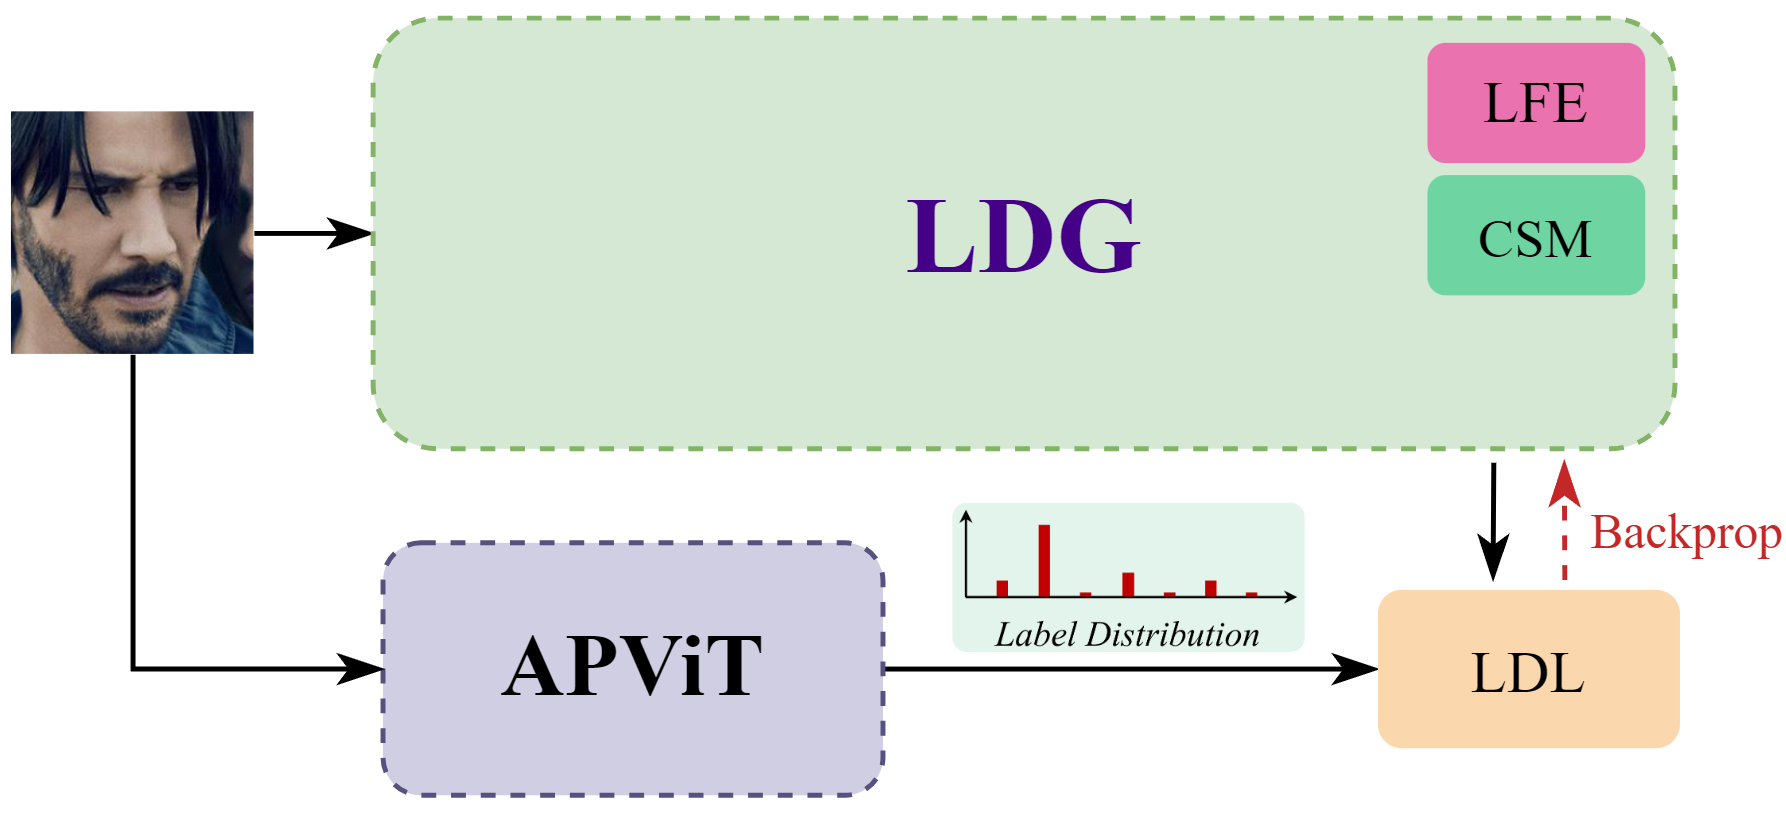
\includegraphics[width=1\columnwidth]{../images/chap_design/Phase 1 diagram.png}
		\caption[Phase I training pipeline]{Training pipeline for the first phase of the proposed algorithm. The IR-50 \cite{deng2019ir50} network is loaded with the backbone weights of APViT \cite{apvit2023} and enhanced with the local-global feature extraction modules from EfficientFace \cite{eff-face2021}. It is then trained using APViT as the distribution generator.}
		\label{fig:phase1-diagram}
	\end{center}
\end{figure}


The modified LDG is based on the same ResNet-50 architecture that serves as the feature extraction backbone of APViT. Three key modifications are proposed to enhance the LDG's FER performance and in turn the performance of the resulting EfficientFace variant. The design for this stage is depicted in figure \ref{fig:phase1-diagram}.

\textbf{1. FER-pretrained backbone weights from APViT:} Instead of initializing the ResNet-50 backbone with ImageNet \cite{deng2009imagenet} pretrained weights (as in the original EfficientFace approach), we initialize it with the backbone weights from a fully trained APViT model. Since APViT uses a hybrid architecture that includes convolutional layers before the transformer encoder, these pretrained weights are already specialized for facial expression recognition. This initialization provides the LDG with feature extractors that are tuned to capture expression-relevant patterns.

\textbf{2. Local-Global feature extraction modules:} We integrate the specialized local-global feature extraction modules from EfficientFace into the modified LDG architecture. These modules are inserted between the convolutional stages of the ResNet-50 backbone, allowing the network to extract both local facial features (such as subtle changes in specific facial regions) and global contextual information (such as overall facial configuration). This architectural enhancement helps the LDG generate more informative label distributions that capture the multi-scale nature of facial expressions.

\textbf{3. Knowledge distillation from APViT:} The modified LDG is trained using knowledge distillation, where the training objective is to minimize the difference between the LDG's output probability distributions and those generated by the fully trained APViT model. Specifically, we employ the same label distribution learning loss from EfficientFace to measure the discrepancy between the two distributions. This training procedure enables the modified LDG to learn to produce soft labels that approximate APViT's predictions while maintaining a more efficient architecture.

\subsubsection{Training EfficientFace with the Modified LDG}

Once the modified LDG is trained, it serves as the label distribution generator for training EfficientFace. The training procedure follows the original label distribution learning approach \cite{eff-face2021}, but with the modified LDG replacing the original ResNet-50 LDG.\\

During EfficientFace training, the modified LDG remains frozen and is used to generate soft label distributions for each training image. EfficientFace is then trained to minimize the loss between its predicted distributions and these soft labels. This two-stage knowledge transfer process, first from APViT to the modified LDG, then from the modified LDG to EfficientFace, should enable the lightweight model to benefit from APViT's superior representational capacity without the computational burden of using APViT directly during training. The design for this stage is depicted in figure \ref{fig:phase2-diagram}.\\

We employ a slightly tweaked version of the EfficientFace source code that fixes some minor bugs and limitations of the original implementation. The modified codebase is publicly available at \url{https://github.com/DavidCrgh/EfficientFace}.


\begin{figure}
	\begin{center}
		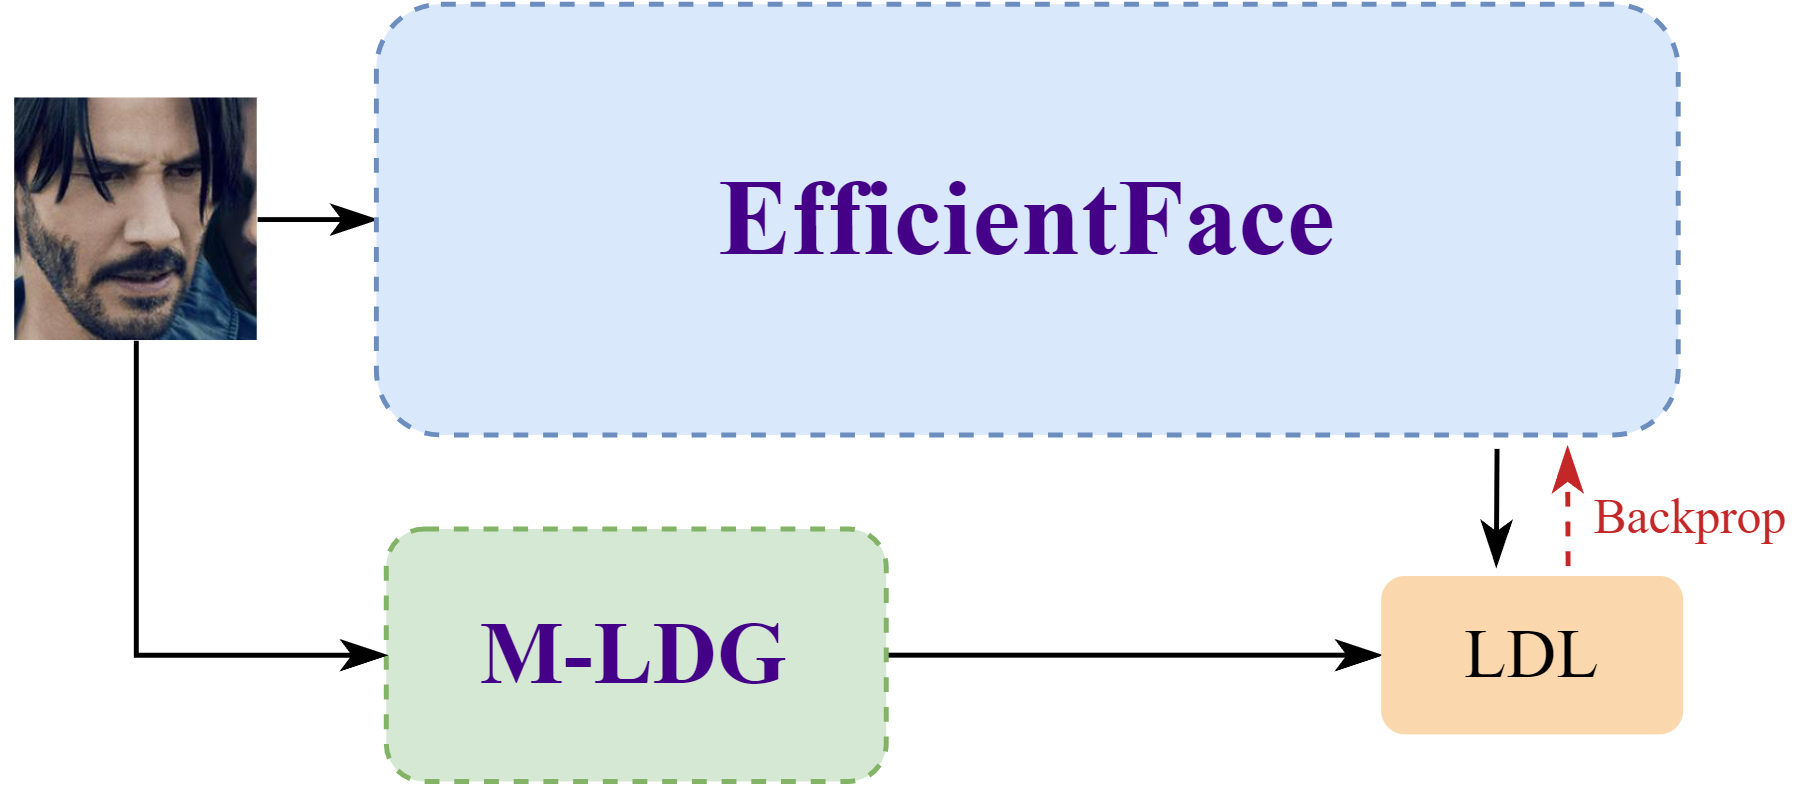
\includegraphics[width=1\columnwidth]{../images/chap_design/Phase 2 diagram.png}
		\caption[Phase II training pipeline]{Training pipeline for the second phase of the proposed algorithm. The modified LDG is used to train EfficientFace on the AffectNet dataset.}
		\label{fig:phase2-diagram}
	\end{center}
\end{figure}

\subsection{Dataset preprocessing}
Dataset preprocessing involves standardizing and transforming the facial images to create model-ready inputs. For each image, the pipeline first detects and aligns faces using RetinaFace \cite{retinaface2020} to account for pose variation and ensure facial landmarks are centered and consistently oriented. Images are then resized and padded to a fixed size of 112 x 112 pixels. These transformations ensure that all images fed to the models are properly aligned, uniformly sized, and consistently formatted, which is critical for robust model training. These steps are carried out once outside the training pipeline.\\

Additional preprocessing steps are applied at training and validation time. These steps follow the exact same procedure as the original EfficientFace architecture. For training, images are first randomly resized and cropped to the target size, followed by random horizontal flipping for data augmentation. Each image is then normalized using mean and standard deviation values matching the ImageNet dataset (mean=[0.485, 0.456, 0.406]; std=[0.229, 0.224, 0.225]). For validation and testing, images are simply resized to the target size, and normalized in the same way, but no random augmentation is applied.

\subsubsection{Image upscaling} \label{section:design-upsampling}
An important implementation detail is that the APViT and modified LDG architectures expect and are trained on 112 x 112 pixel images as input, while EfficientFace expects 224 x 224 sized images. To address this, we upscale the images to 224 x 224 during training in the second phase of the proposed algorithm. The upscaling is carried out using bilinear interpolation.

\subsection{Hyperparameter optimization}

Both phases of the experimental design follow the same general procedure. First, the experiment is executed across all factor combinations. From these runs, the best-performing combinations are selected and subjected to hyperparameter optimization. The optimization searches over learning rate, momentum, weight decay, and the learning rate schedule (adjustment frequency and reduction factor), using a Bayesian search with early termination (Hyperband \cite{hyperband2018}) to select the best configuration. The resulting optimized model is taken as the winner or representative of that phase. Phase II uses the Phase I winner whenever the modified LDG is the selected guidance network: the best modified LDG from Phase I is loaded as the frozen label distribution generator for training EfficientFace in the corresponding Phase II condition.

\subsection{Training APViT on AffectNet}\label{section:design-apvit-training}

As noted in the Requirements section, pretrained APViT weights for AffectNet were not publicly available at the time of this work. The network was therefore trained from scratch following the procedure described in the original APViT paper \cite{apvit2023}.\\

The public APViT codebase is oriented toward training on the RAF-DB dataset, so modifications were necessary to support training on AffectNet. These adaptations include changes to the data loading pipeline, class configuration, and evaluation scripts. The modified codebase is publicly available at \url{https://github.com/DavidCrgh/APViT}.\\

Table~\ref{tab:design-apvit-hyperparams} lists the key training hyperparameters used for this run. These values were taken directly from the configuration file provided in the original repository and kept unchanged.\\

\begin{table}[h]
    \centering
    \caption[APViT training hyperparameters for AffectNet]{APViT training hyperparameters used for training on AffectNet.}
    \label{tab:design-apvit-hyperparams}
    \begin{tabular}{ll}
        \toprule
        \textbf{Hyperparameter} & \textbf{Value} \\
        \midrule
		Training iterations (batches) & 6000 \\
        Input image size       & 112$\times$112 px \\
        Batch size             & 128 \\
        Optimizer              & SGD \\
        Learning rate          & $5 \times 10^{-4}$ \\
        Momentum               & 0.9 \\
        Weight decay           & $5 \times 10^{-4}$ \\
        LR schedule            & Cosine Annealing \\
        Gradient clip max norm & 10.0 \\
        ViT depth              & 8 layers \\
        ViT embedding dim      & 768 \\
        Attention heads        & 8 \\
        CNN pool (patches retained) & 160 \\
        \bottomrule
    \end{tabular}
\end{table}

The trained APViT achieved 64.2\% accuracy on AffectNet-7 and 57.31\% on AffectNet-8. These results are below the 66.91\% reported in the original paper \cite{apvit2023}, which was obtained on the same AffectNet-7 split, suggesting there is room for further tuning. Nevertheless, the trained model provides a functional teacher network for the proposed knowledge distillation pipeline.

\subsection{Limitations and Requirements}

This section outlines the key limitations and requirements of our proposed design, derived from the scope and limitations defined for this research project.

\subsubsection{Limitations}

Refer to section \ref{section:scope-limitations} for the limitations of this research project.

\subsubsection{Requirements}

\textbf{Pretrained models:} \label{section:design-pretrained-models} The proposed approach requires access to model weights for the APViT network pretrained on the AffectNet dataset. To the best of our knowledge, these weights are not publicly available. As such, we retrained the network from scratch using the same procedure as described in the original APViT paper \cite{apvit2023}.

\textbf{Computational resources:} The main computational resource required for executing the proposed approach is the available GPU memory. Phase I of the design requires more memory since it leverages the two heaviest networks: APViT and the modified LDG. In executions of Phase I, we noticed a memory requirement of approximately 16GB of VRAM per training run.

\textbf{Dataset access:} The execution of the proposed approach requires access to the 7-class and 8-class subsets of the AffectNet dataset \cite{affnet2019}.

\textbf{Software environment:} Execution of the training scripts requires an environment with the following software:
\begin{itemize}
    \item Python 3.10
    \item PyTorch 1.11 and CUDA 11.8
    \item MMCV 1.7.1
    \item WandB
    \item RetinaFace \cite{retinaface2020}
    \item A copy of the main code repository. (See \ref{section:implementation}).
\end{itemize}

\textbf{Face alignment tools:} The main code repository contains a script for face alignment using RetinaFace. Any of its dependencies must be installed in the execution environment.

\subsection{Implementation}\label{section:implementation}

The main code repository is hosted on GitHub and can be accessed at the following URL: \url{https://github.com/DavidCrgh/FER-MLDG}. The \texttt{src/networks} directory contains the implementations of the APViT, LDG, and EfficientFace architectures. Dataset preprocessing code, including face alignment with RetinaFace and conversion to the formats required by each network, is located in the \texttt{src/preproc} directory. Experiment execution is organized through Jupyter notebooks. The notebooks handle environment setup, configuration loading, and invocation of the underlying training scripts. Notebooks are also provided for executing the hyperparameter optimization process using WandB Sweeps.